\documentclass[class=book, crop=false, oneside]{standalone}
\usepackage[subpreambles=true]{standalone}

\usepackage{../../style}

\graphicspath{{./assets/images/}}
\newmintinline{asm}{}

% arara: pdflatex: { synctex: yes, shell: yes }
% arara: latexmk: { clean: partial }
\begin{document}
\chapter{Pipeline}

\section{Introduzione}
Nel capitolo precedente è stato presentato lo schema base di un semplice processore che esegue un'operazione per ogni ciclo di clock, tuttavia questo \emph{modus operandi} è molto svantaggioso in quanto il clock deve essere calibrato in base alla durata delle operazioni più lente. Quindi, se si implementano istruzioni complesse, questo rallenta di molto la velocità del clock e di conseguenza quella del processore stesso, che dovrà aspettare la durata di un clock intero anche per istruzioni molto semplici che richiedono meno tempo. Tutto ciò rende impossibile compiere ottimizzazioni aggressive sulle operazioni più comuni.

Esistono, tuttavia, dei procedimenti che permettono di migliorare il rendimento della CPU.
Uno dei metodi più semplici è quello di parallelizzare il lavoro, in una maniera molto simile a quella con cui Henry Ford migliorò la produzione delle fabbriche del primo Novecento.

Il punto centrale di questa strategia sta nel comprendere che mentre una componente della CPU sta lavorando sull'istruzione corrente, un'altra componente può iniziare a svolgere l'istruzione successiva; in tal modo lo svolgimento delle operazioni non è più prettamente sequenziale ma diventa parallelo, in un certo senso, perché lo svolgimento di un'operazione avviene nello stesso momento dello svolgimento di un'altra, anche se le due operazioni si trovano in fasi di completamento diverse.

Una misura del miglioramento che si introduce con metodi come il lavoro in parallelo è data dal \emph{throughput}, il quale è definito come il numero di operazioni risolte per unità di tempo. In una catena di lavoro in parallelo composta da \(n\) stadi il \emph{throughput} massimo raggiungibile è \(\frac{1}{n}\); si intuisce che con un meccanismo di lavoro in parallelo ben funzionante a regime si possono fare \(n\) operazioni nello stesso tempo in cui normalmente se ne fa una sola, e questo è un miglioramento notevole.

\subsection*{Pipeline}
Il concetto di pipeline è esattamente simmetrico a quello di catena di montaggio: viene detta pipeline un'implementazione della CPU che prevede lo svolgimento di più operazioni in parallelo.

Tornando al caro vecchio MIPS, ricordiamo brevemente quali sono le fasi per l'esecuzione di un'istruzione:
\begin{enumerate}[noitemsep]
	\item fetch;
	\item lettura registri e decodifica dell'istruzione;
	\item esecuzione di un'operazione (di tipo R) o calcolo di un indirizzo;
	\item accesso ad un operando nella memoria dati (nel caso di \opcode{lw} o \opcode{sw});
	\item scrittura del risultato in un registro (\emph{writeback}).
\end{enumerate}
\begin{figure}[H]
	\centering
	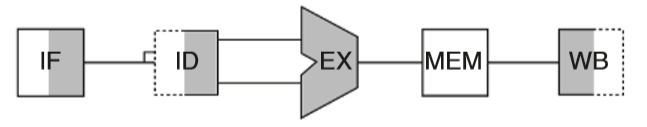
\includegraphics[width=.5\textwidth,keepaspectratio]{istruzione.png}
	\caption{IF sta per instruction fetch, ID per instruction decode, EX per execution, MEM per accesso alla memoria dati e WB per \emph{writeback}}
\end{figure}
Dunque, avendo un processo suddiviso in \(5\) step, la pipeline che useremo per parallelizzare il lavoro della CPU sarà composta da \(5\) stadi.

\section{Esempio}
Per comprendere meglio il concetto è presentato di seguito un esempio semplificato di pipeline, in cui le uniche operazioni possibili sono:
\begin{itemize}
	\item \opcode{lw} e \opcode{sw} di accesso alla memoria;
	\item \opcode{and}, \opcode{or} e \opcode{slt} di tipo R;
	\item \opcode{beq} di tipo salto.
\end{itemize}
Naturalmente i tempi necessari per l'esecuzione di queste operazioni non sono uguali: è riportata quindi una tabella con annessi i tempi di esecuzione (veri solo nel nostro esempio) relativi ad ogni categoria di operazione.
\begin{figure}[H]
	\centering
	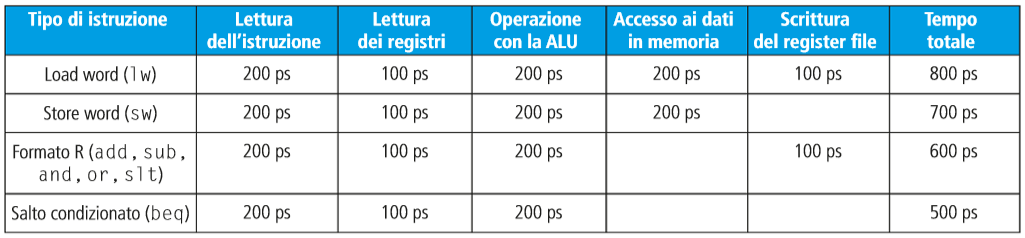
\includegraphics[width=\textwidth,keepaspectratio]{tabella-tempi-operazioni.png}
	\caption{Tempi d'esecuzione per ciascuna fase (nel nostro esempio)}
\end{figure}
Si noti che l'istruzione più lenta di tutte è la \texttt{load word}\footnote{Si noti anche che questa è l'unica istruzione che esegue effettivamente tutte le 5 fasi descritte in precedenza.}; di conseguenza il tempo di clock viene stabilito in base ad essa.

Inoltre il tempo dedicato ad ogni singola fase del processo di esecuzione è definito in base al tempo della fase con durata massima, ovvero nel nostro caso \unit[200]{ps}, per rendere possibile il partizionamento in fasi della stessa durata (altrimenti il parallelismo non sarebbe possibile).
Questo tuttavia implica che anche le fasi con durata inferiore verranno eseguite in un tempo di \unit[200]{ps} ed anche che la durata dell'esecuzione di una singola istruzione nella nostra pipeline è di \((\textrm{tempo singola fase})*(\textrm{numero fasi})=200ps\cdot 5=1000ps\).

Osserviamo quindi un diagramma temporale per sequenza istruzioni in cui si confronta lo svolgimento di operazioni con il metodo standard e attraverso l'implementazione della pipeline.
\begin{figure}[H]
	\centering
	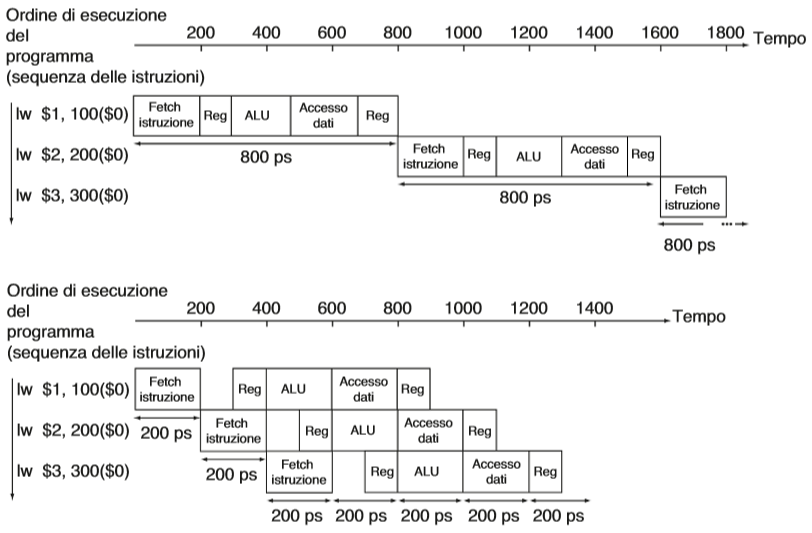
\includegraphics[width=\textwidth,keepaspectratio]{esecuzione-operazioni-confronto.png}
	\caption{\label{esempioPipeline}Il grafico in alto raffigura la normale esecuzione di un programma, il grafico sotto invece rappresenta lo svolgimento dello stesso con il meccanismo della pipeline; si noti che la fase reg è forzatamente fatta durare 200ps, ed inoltre si noti di quanto è ridotta la durata del programma.}
\end{figure}

\subsection{Osservazioni}
La teoria prevede che per avere una stima delle prestazioni della CPU una volta implementata una pipeline si possa usare la seguente formula:
\begin{equation*}
\text{Tempo tra due istruzioni con pipeline} = \frac{\text{Tempo tra due istruzioni senza pipeline}}{\text{Numero di stadi della pipeline}}
\end{equation*}
Quindi teoricamente, secondo questa formula, nel nostro caso ci si aspetta un miglioramento delle prestazioni di un fattore 5; tuttavia si può notare nell'esempio in figura \ref{esempioPipeline} che il tempo per eseguire 3 istruzioni passa da \unit[2400]{ps} a \unit[1400]{ps}, generando quindi un miglioramento di un fattore \(1.7\).

Le cause di questa discrepanza sono principalmente due: in primis si deve sottolineare che per ottenere una prestazione 5 volte più alta il tempo di clock dovrebbe essere uguale a quelo di una singola fase del ciclo, ovvero \(\frac{800}{5}=\) \unit[160]{ps}, mentre nella realtà non possiamo scendere sotto ai \unit[200]{ps} poiché ci sono delle fasi che hanno tale durata e quindi impongono un limite minimo alla durata di una fase. In secondo luogo abbiamo considerato poche istruzioni e questo implica che non abbiamo fatto in tempo a distribuire il costo di "avvio" e di "terminazione" della pipeline (i due periodi in cui la pipeline non è completamente a regime); il miglioramento si osserva meglio quando il numero di istruzioni è ben più alto del numero delle fasi della pipeline.

\section{Vantaggi del RISC}
L'architettura di tipo RISC presenta dei vantaggi sostanziali per quanto riguarda il processo di \emph{pipelining}, i principali sono riassunti nell'elenco sottostante.
\begin{itemize}
	\item Tutte le istruzioni hanno la stessa lunghezza, cosa che facilita di molto il prelievo, dal momento che si lavora sempre su word di dimensione fissata.
	\item I codici degli operandi sono in posizione fissa, questo permette di accedervi leggendo il file register in parallelo con la decodifica dell’istruzione.
	\item Gli operandi residenti in memoria sono possibili solo per \opcode{lw} e \opcode{sw}. Ciò permette di usare la ALU per il calcolo di indirizzi, cosa che non sarebbe possibile se dovessimo usare le ALU in due fasi della stessa istruzione, come invece richiesto in ISA più complesse.
	\item  L’uso di accessi allineati fa sì che gli accessi in memoria avvengano sempre in un ciclo di trasferimento, impegnando quindi un solo stadio della pipeline.
\end{itemize}

\section{Condizioni di Hazard}
In condizioni normali una pipeline permette di eseguire un'istruzione per ciclo di clock, ma questo non è sempre possibile, soprattutto quando si verificano delle determinate condizioni critiche dette \emph{hazard}. Ne esistono diversi tipi:
\begin{itemize}
	\item hazard \emph{strutturali};
	\item hazard \emph{sui dati};
	\item hazard \emph{sul controllo}.
\end{itemize}
Osserviamo quindi come vengono a verificarsi queste condizioni critiche e quali sono le soluzioni più comuni adottate per risolverle.

\subsection{Hazard strutturale}
Una condizione di hazard strutturale è una condizione che si verifica quando l'architettura dell’elaboratore rende impossibile l’esecuzione di alcune sequenze di istruzioni in pipeline. Ad esempio, se si disponesse di un'unica memoria, non si potrebbe nello stesso ciclo di clock caricare istruzioni e memorizzare (o prelevare) operandi dalla memoria: è proprio per questa ragione che la memoria dati è separata dalla memoria istruzioni.

\subsection{Hazard sui dati}
Per spiegare questo hazard ricorriamo al seguente esempio di codice MIPS:
\begin{minted}[linenos]{asm}
add $s0, $t0, $t1
sub $t2, $s0, $t3
\end{minted}
Andando ad analizzare come la pipeline implementerebbe questo codice si nota che \register{\$s0} viene salvato nella quinta fase di \opcode{add}, ma lo stesso registro è necessario nella seconda fase di \opcode{sub}; volendo implementare la pipeline si dovrebbe lasciare il processore in stallo per il tempo necessario per la memorizzazione di \register{\$s0}.

Esistono dei metodi per evitare queste tre intere fasi di attesa: il più semplice (e spesso anche il più funzionale) prevede un rimescolamento delle istruzioni. Esso consiste nell'allontanare tra loro le due istruzioni quanto basta per far sì che la prima termini in tempo per garantire la corretta esecuzione della seconda; tuttavia questa strada non è sempre percorribile.

Quella appena descritta è una delle operazioni che compilatori come il \texttt{gcc} compiono nella fase di traduzione da linguaggio ad alto livello ad Assembly. Una soluzione ancora più efficiente è quella dell'\emph{operand forwarding} (detto anche propagazione o bypass): questa in casi come questo prevede di rendere il contenuto del registro \register{\$s0} disponibile per l'operazione successiva ancora prima che questo sia effettivamente salvato nel registro stesso, dato che quel valore sarà già noto dalla fase "execute" dell'istruzione \opcode{add}.
Si osservi lo schema riportato qui sotto per una maggiore comprensione del meccanismo di propagazione.
\begin{figure}[H]
	\centering
	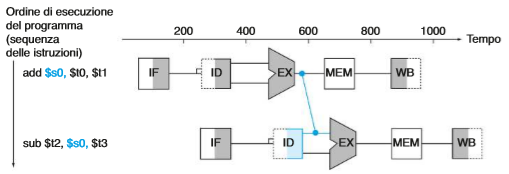
\includegraphics[width=.8\textwidth,keepaspectratio]{propagazione.png}
	\caption{Meccanismo dell'operand forwarding}
\end{figure}

\subsection{Hazard sul controllo}
Questo tipo di hazard riguarda nello specifico le operazioni di salto condizionato, che generano problemi in quanto prima dell'effettivo termine della loro esecuzione non si può sapere quale sarà l'istruzione sucessiva. Se la pipeline è composta da tante fasi il tempo che si aspetterebbe prima di sapere come procedere potrebbe diventare eccessivo.

Per il resto del capitolo consideriamo di avere un circuito molto sofisticato che ci permette di calcolare l’indirizzo di salto già al secondo stadio (ID); tuttavia questo non basta poiché dobbiamo lasciare la pipeline in stallo per almeno una fase prima di sapere qual è l'istruzione successiva. Esistono tre tipi di soluzione all'hazard sul controllo, e sono riportate in seguito in ordine di complessità.

\begin{enumerate}
	\item Il primo approccio prevede di risistemare l'ordine delle istruzioni (come si farebbe per risolvere un hazard sui dati) facendo eseguire subito dopo il branch delle istruzioni indipendenti dal salto stesso, che quindi dovrebbero essere eseguite indifferentemente; questo metodo è molto comodo, ma purtroppo non è sempre applicabile.
	\item Il secondo approccio viene chiamato \emph{untaken branch} e consiste nel considerare sempre che il salto non si verifichi e far quindi proseguire la pipeline regolarmente nell'esecuzione delle operazioni. Quando invece la condizione di salto viene verificata ci sono due casi: se il salto non deve avvenire allora il problema si è risolto da solo e la pipeline può proseguire tranquillamente il suo lavoro, altrimenti si deve ripristinare lo stato del processore a quello precedente all'istruzione del salto, questa volta eseguendo il salto stesso. Questo implica la necessità di creare dei \emph{registri di backup} dove si va a salvare per l'appunto lo stato del processore ogni volta che si esegue il fetch di un'operazione di salto condizionale.
	\item Il terzo approccio è una versione più raffinata del secondo, in cui è prevista l'implementazione di una circuiteria di \emph{branch prediction}, che serve appunto per dare una stima della probabilità con cui avverrà il salto; questo permette di avere dei miglioramenti sull'efficienza del meccanismo \emph{untaken branch}. Un circuito di \emph{branch prediction} calcola a runtime la probabilità con cui si verificherà un salto condizionale e può decidere se settare il comportamento standard come \emph{untaken branch} o come \emph{taken branch}. Se ad esempio un programma prevede che un ciclo venga eseguito 1000 volte il circuito di \emph{branch prediction} dopo qualche ripetizione setterà la risposta standard a \emph{taken branch} e quindi risparmierà molte fasi di ripristino dello stato della CPU dovute ad errori di predizione (che sarebbero avvenuti con certezza usando il meccanismo \emph{untaken branch}).
\end{enumerate}

\subsection{Registri di backup}
Come detto in precedenza, per meccanismi come l'\emph{untaken branch} e l'implementazione di circuiti di \emph{branch prediction} si rendono necessari dei registri da utilizzare come backup dello stato del processore nel caso la predizione effettuata si riveli errata. Nell'immagine presente qui sotto si possono osservare tali registri; si noti che il nome dei registri viene dato a seconda delle fasi che separano (information fetch/information decode/execute...).
\begin{figure}[H]
	\centering
	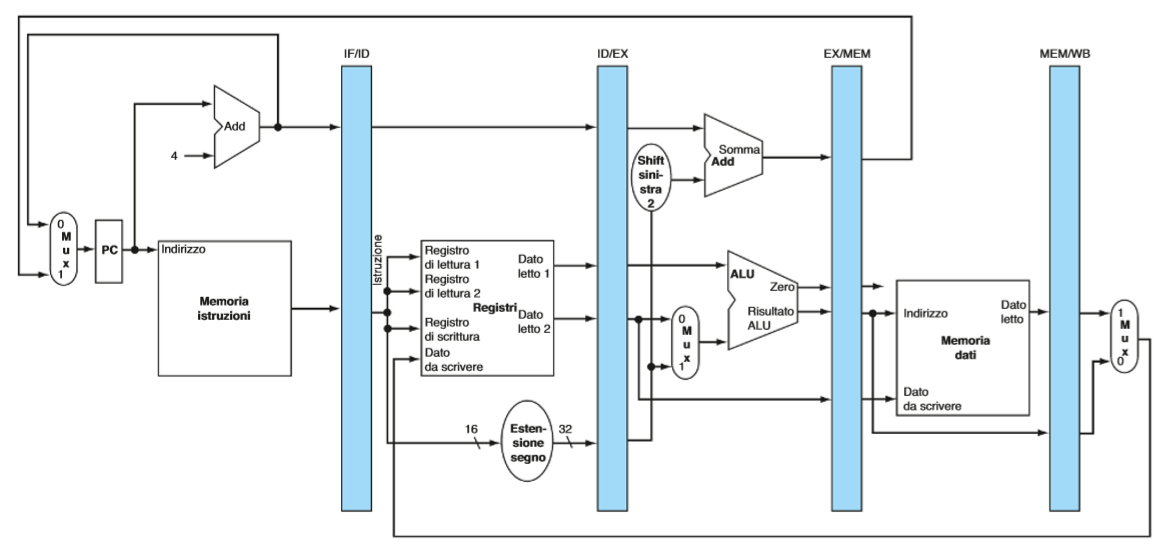
\includegraphics[width=\textwidth,keepaspectratio]{registri-di-backup.png}
\end{figure}
Un altro aspetto particolare di questa componente riguarda le dimensioni che i registri di backup devono avere: queste infatti sono molto variabili e dipendono strettamente da cosa il registro in causa deve memorizzare. Il registro IF/ID, per esempio, deve contenere 64 bit, 32 per l’istruzione prelevata dalla memoria ed altri 32 per il contenuto del PC incrementato di 4. Gli altri tre registri di pipeline contengono rispettivamente 128, 97 e 64 bit.

\section{Esercizio tipo}
È qui riportato un esempio di possibile esercizio da esame riguardante questi argomenti.
Si consideri una CPU che impiega \unit[600]{ps} per la fase di fetch, \unit[600]{ps} per la fase di decodifica, \unit[500]{ps} per eseguire operazioni con la ALU, \unit[400]{ps} per la fase di accesso alla memoria e \unit[700]{ps} per la fase di scrittura nel register file.

Qual è il massimo incremento che ci si può attendere usando una pipeline?
Per prima cosa si calcola il tempo totale di un'operazione senza pipeline:
\begin{equation*}
	\text{Tempo totale} = 600+600+500+400+700 = 2800ps
\end{equation*}
In seguito si ricorda che il tempo di clock una volta implementata la pipeline sarà uguale al tempo della fase con durata più lunga, ovvero nel nostro caso \unit[700]{ps}. Dunque il tempo di esecuzione di una singola operazione sarà ridotto (tramite il parallelismo, quindi virtualmente) a: \(\frac{\text{Tempo totale}}{\text{Operazione più lenta}}\). Ciò significa che l'incremento delle prestazioni si calcolerà come segue:
\begin{equation*}
	\text{Incremento} = \frac{\text{Tempo totale}}{\text{Operazione più lenta}} = \frac{2800}{700} = 4
\end{equation*}
ovvero l'incremento finale sarà di 4 volte.

\end{document}
